\chapter{Experiments}\label{r:experiments}

This chapter presents a comprehensive experimental evaluation of proposed \method{} framework for generating \framework{}. This work systematically evaluates the method's ability to generate diverse, high-quality samples while maintaining invariant set membership across three complementary experimental paradigms: individual neuron activation analysis, sparse autoencoder (SAE) feature investigation, and classifier output preservation.

\section{Experimental Design}

The experimental evaluation systematically investigates the capabilities and limitations of the proposed framework through a comprehensive analysis that spans multiple scales of neural network representation. The evaluation begins by examining whether \method{} can generate visually diverse samples that maintain identical activation patterns for interpretable neurons, thereby establishing the method's precision in preserving specific neural responses while exploring the complete space of visual inputs that trigger identical activations. This initial investigation focuses on establishing the fundamental capability of the framework to maintain mathematical precision in activation preservation while simultaneously generating semantically meaningful variations that extend beyond typical training data examples.

Building upon this foundation, the evaluation proceeds to examine whether generated samples can reveal semantic patterns that transcend those present in conventional training datasets. This investigation addresses a fundamental limitation in current interpretability research, where understanding of neural network representations remains constrained by the statistical biases and limited scope of training data. The framework's ability to generate novel visual patterns that maintain identical neural responses provides unprecedented insight into the true representational capacity of learned features, revealing semantic concepts and visual patterns that remain hidden when analysis is restricted to naturally occurring dataset examples.

The evaluation framework extends beyond individual neuron analysis to encompass more sophisticated learned representations through investigation of sparse autoencoder features. These features represent hierarchical and compositional visual patterns that capture complex structural relationships within neural network representations. The preservation of these multi-dimensional feature activations presents significantly greater computational and theoretical challenges than individual neuron targeting, requiring simultaneous maintenance of activation patterns across multiple learned components while preserving the semantic coherence of generated samples.

The most comprehensive and challenging aspect of the evaluation addresses the framework's ability to maintain complete classifier predictions while generating semantically meaningful variations. This investigation represents the ultimate test of invariant set generation capabilities, as it requires preserving entire output distributions rather than individual activation components. The successful preservation of classifier outputs while generating diverse visual samples demonstrates the framework's capacity to navigate complex high-dimensional decision boundaries while maintaining both mathematical precision and semantic meaningfulness. This comprehensive evaluation establishes a rigorous assessment framework that spans from individual computational units to complete model behaviors, providing thorough validation of the proposed approach across multiple scales of neural network analysis.

\subsection{Infrastructure and Implementation}

All experiments were conducted on NVIDIA A100 GPUs (1-4 units) using PyTorch. This work employs LightningDiT as proposed diffusion backbone with SGD optimization at learning rate $\eta = 10$ based on empirical hyperparameter evaluation (see \cref{appendix:hyperparameters}). Each experimental condition generates 32-256 samples due to computational constraints, representing a balance between statistical validity and resource efficiency.

\subsection{Evaluation Framework}

This work employs a multi-faceted evaluation approach combining quantitative precision metrics with qualitative semantic analysis to comprehensively assess both the mathematical rigor and semantic meaningfulness of generated invariant sets.

\textbf{Quantitative Metrics:} The quantitative evaluation framework encompasses three complementary measurement approaches that collectively establish the mathematical precision and statistical validity of generated samples. 

\textbf{Activation Fidelity Assessment} employs $L_2$ norm deviations from target values to quantify the precision of constraint satisfaction. The $L_2$ distance between target and generated activations is computed as:
\begin{equation}
\mathcal{L}_{\text{L2}} = \|n(\mathbf{x}) - n(\mathbf{x^*})\|_2 = \sqrt{\sum_{i=1}^{d}(n_i(\mathbf{x}) - n_i(\mathbf{x^*}))^2}
\end{equation}
where $n(\mathbf{x})$ represents the neural network activation vector for input $\mathbf{x}$, $n(\mathbf{x^*})$ denotes the target activation pattern, and $d$ is the dimensionality of the activation space. The $L_2$ norm provides sensitivity to large deviations in activation patterns while maintaining mathematical tractability for gradient-based optimization. This metric serves as the primary constraint satisfaction measure, with values below 1.0 indicating excellent preservation of target neural responses. The choice of $L_2$ over $L_1$ norms stems from its differentiability properties and its alignment with the Euclidean geometry of high-dimensional activation spaces, facilitating stable optimization convergence during invariant set generation.

\textbf{FID and sFID (realism).} Following works on image synthesis, measuring the realism of the obtained explanations at a distribution level is often done with FID and sFID. Specifically, FID compares a set of real (\emph{r}) and generated (\emph{g}, in this case, the explanations) images by first extracting their corresponding features from the InceptionV3 network and then computing:
\begin{equation}
\text{FID} = ||\boldsymbol{\mu}_r - \boldsymbol{\mu}_g||^2 + \text{Tr}\left( \Sigma_r + \Sigma_g - 2\left(\boldsymbol{\Sigma}_r \boldsymbol{\Sigma}_g \right)^{1/2} \right),
\end{equation}
where $\boldsymbol{\mu}_r, \boldsymbol{\mu}_g$ are the mean vectors and $\boldsymbol{\Sigma}_r, \boldsymbol{\Sigma}_g$ are the covariance matrices of the respective distributions in the feature space. The FID metric quantifies distributional similarity between generated and natural images through comparison of their statistical moments in the InceptionV3 feature space. The first term $||\boldsymbol{\mu}_r - \boldsymbol{\mu}_g||^2$ measures the squared Euclidean distance between distribution means, capturing differences in average feature activations. The second term involving the trace operation measures the difference in covariance structures, quantifying how feature correlations differ between real and generated image sets. As comparing original images with their edited versions (e.g., explanations) may bias the metric with original pixels mostly unchanged, artificially boosting the realism evaluation, sFID first divides the sets into folds and averages FID over the independent counterparts. This approach provides a robust measure of visual quality that correlates strongly with human perceptual judgments while remaining sensitive to subtle artifacts that might compromise the naturalistic appearance of generated samples.

\textbf{Spectral Coherence Analysis} employs frequency domain examination using ideal low-pass filters to ensure that generated samples achieve invariance through semantically meaningful rather than imperceptible high-frequency variations, distinguishing the approach from adversarial methods that exploit human visual system limitations. This analysis applies a series of low-pass filters with varying cutoff frequencies to generated samples, measuring how invariant set membership degrades as high-frequency components are progressively removed. Robust invariant set membership under spectral filtering indicates that activation preservation relies on semantic content rather than adversarial perturbations, providing critical validation that generated variations represent genuine semantic diversity rather than exploitation of network vulnerabilities.

\textbf{Qualitative Assessment:} The qualitative evaluation framework focuses on three critical dimensions that capture the semantic validity and interpretability implications of generated invariant sets. Semantic diversity assessment within invariant sets evaluates whether generated samples reveal broader representational capacities than apparent from typical training data, examining the range of visual concepts, compositional variations, and stylistic differences that maintain identical neural responses while expanding understanding of learned feature selectivity.

Visual coherence evaluation and adversarial artifact detection ensure that generated samples maintain naturalistic appearance and avoid the characteristic distortions associated with adversarial perturbations, distinguishing semantically meaningful variations from artificial manipulations that exploit network vulnerabilities. This assessment includes examination of edge consistency, texture regularity, lighting coherence, and overall photorealistic quality to confirm that invariant set membership is achieved through genuine semantic diversity rather than imperceptible but systematic distortions.

\subsection{Critical Motivation: Dataset Bias and Synthetic Data Necessity}

\textbf{Neuron labeling doesn't work.} Traditional approaches to neural network interpretability that rely solely on natural dataset analysis face fundamental limitations due to systematic dataset biases that obscure the true representational capacity of learned features. Conventional neuron labeling methodologies, which attempt to characterize neural function based on naturally occurring activation patterns, fail to capture the complete scope of visual patterns that can trigger identical neural responses.

\textbf{You must generate synthetic data because the dataset is biased.} The necessity for synthetic data generation stems from the inherent limitations of training datasets, which represent only a narrow subset of the complete visual manifold that neural networks can process. These datasets exhibit systematic biases in visual composition, semantic coverage, and statistical properties that prevent comprehensive understanding of learned representations. Natural datasets contain correlated features, missing visual patterns, and skewed distributions that mask the true decision boundaries and feature selectivity of trained models.

\begin{figure}[h]
\centering
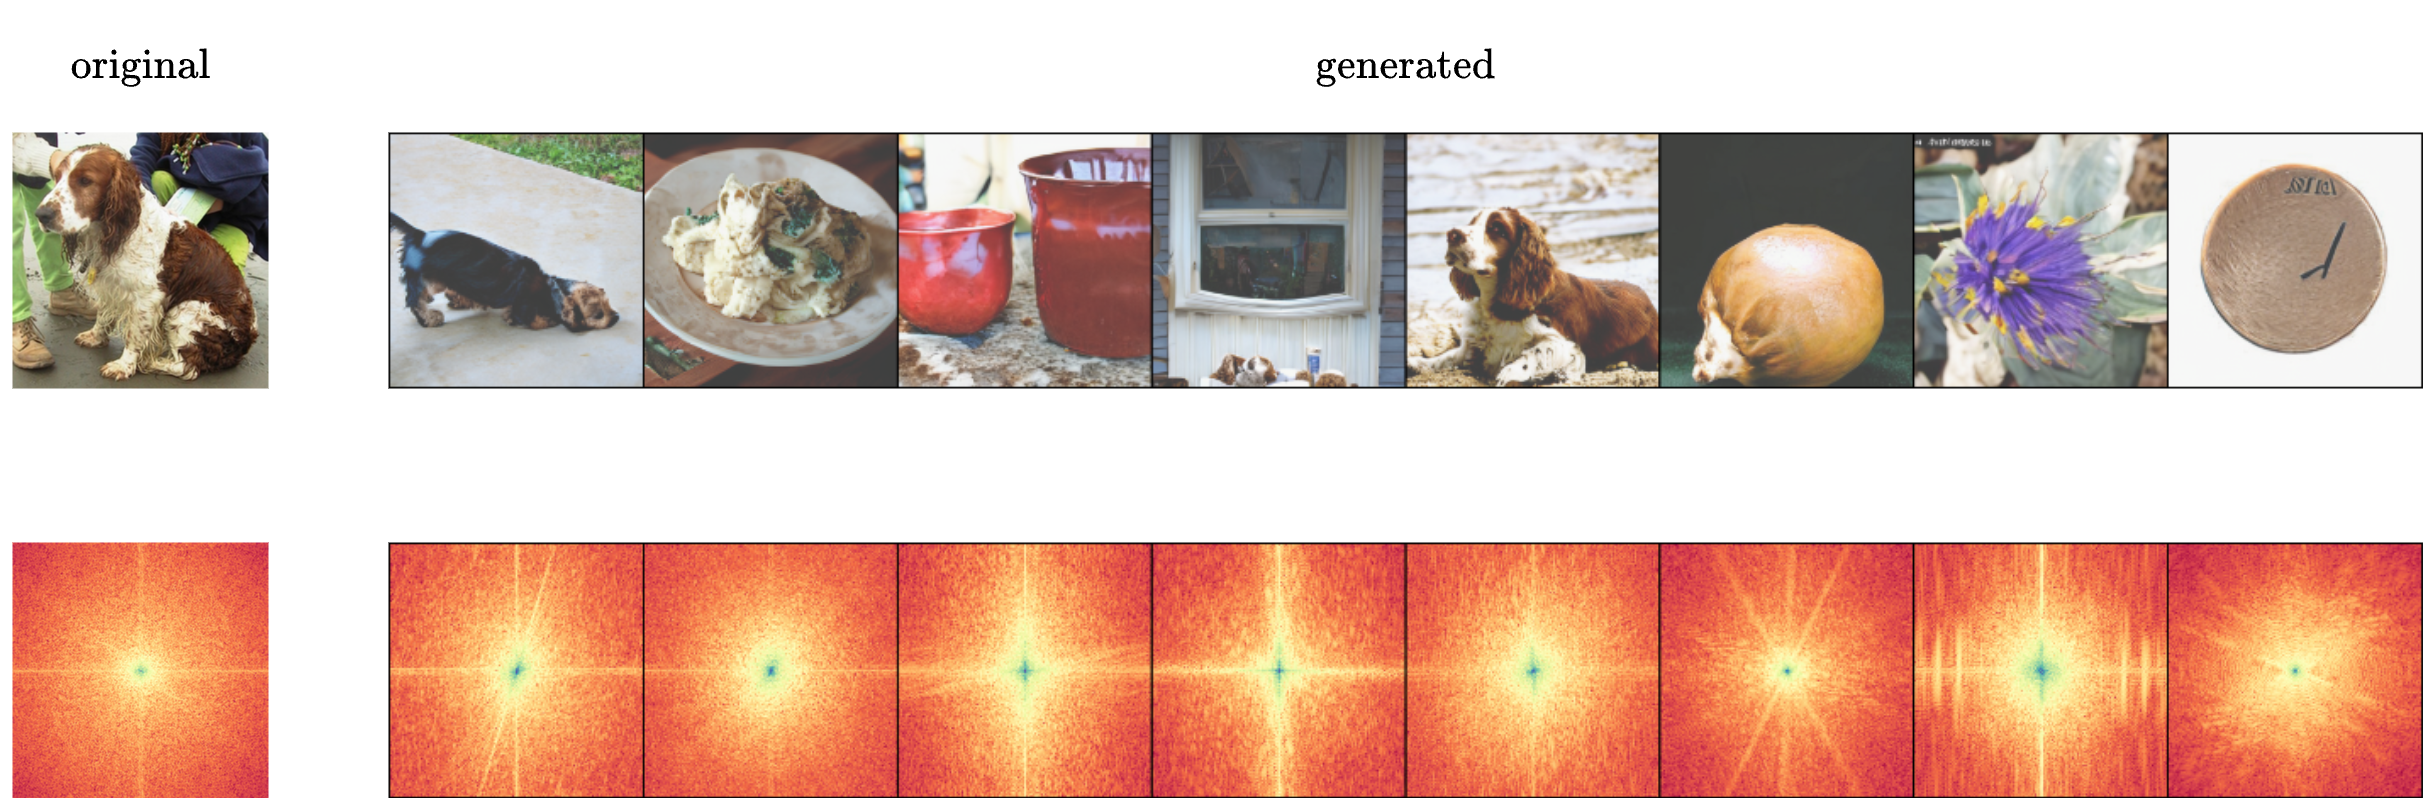
\includegraphics[width=\linewidth]{figures/main/spectral_analysis_1.png}
\caption{\textbf{Critical evidence: Natural datasets are insufficient for understanding neural representations.} Invariant images that preserve ResNet50 classifier probability with ~0.01 L2 loss on the right and original image on the left. Bottom row shows 2D spectral heatmap computed via $|\mathcal{F}(\mathbf{x})(u,v)|^2$ where $\mathcal{F}(\mathbf{x})$ represents the discrete Fourier transform and $(u,v)$ denote frequency coordinates, revealing power distribution across spatial frequencies. Although generated samples are of high quality, this frequency domain analysis can detect their synthetic nature through distinct spectral signatures. This demonstrates that neural networks respond to visual patterns that exist beyond the limited scope of natural training data, making synthetic data generation essential for comprehensive interpretability analysis.}
\label{fig:dataset_bias_evidence}
\end{figure}

\begin{figure}[h]
\centering
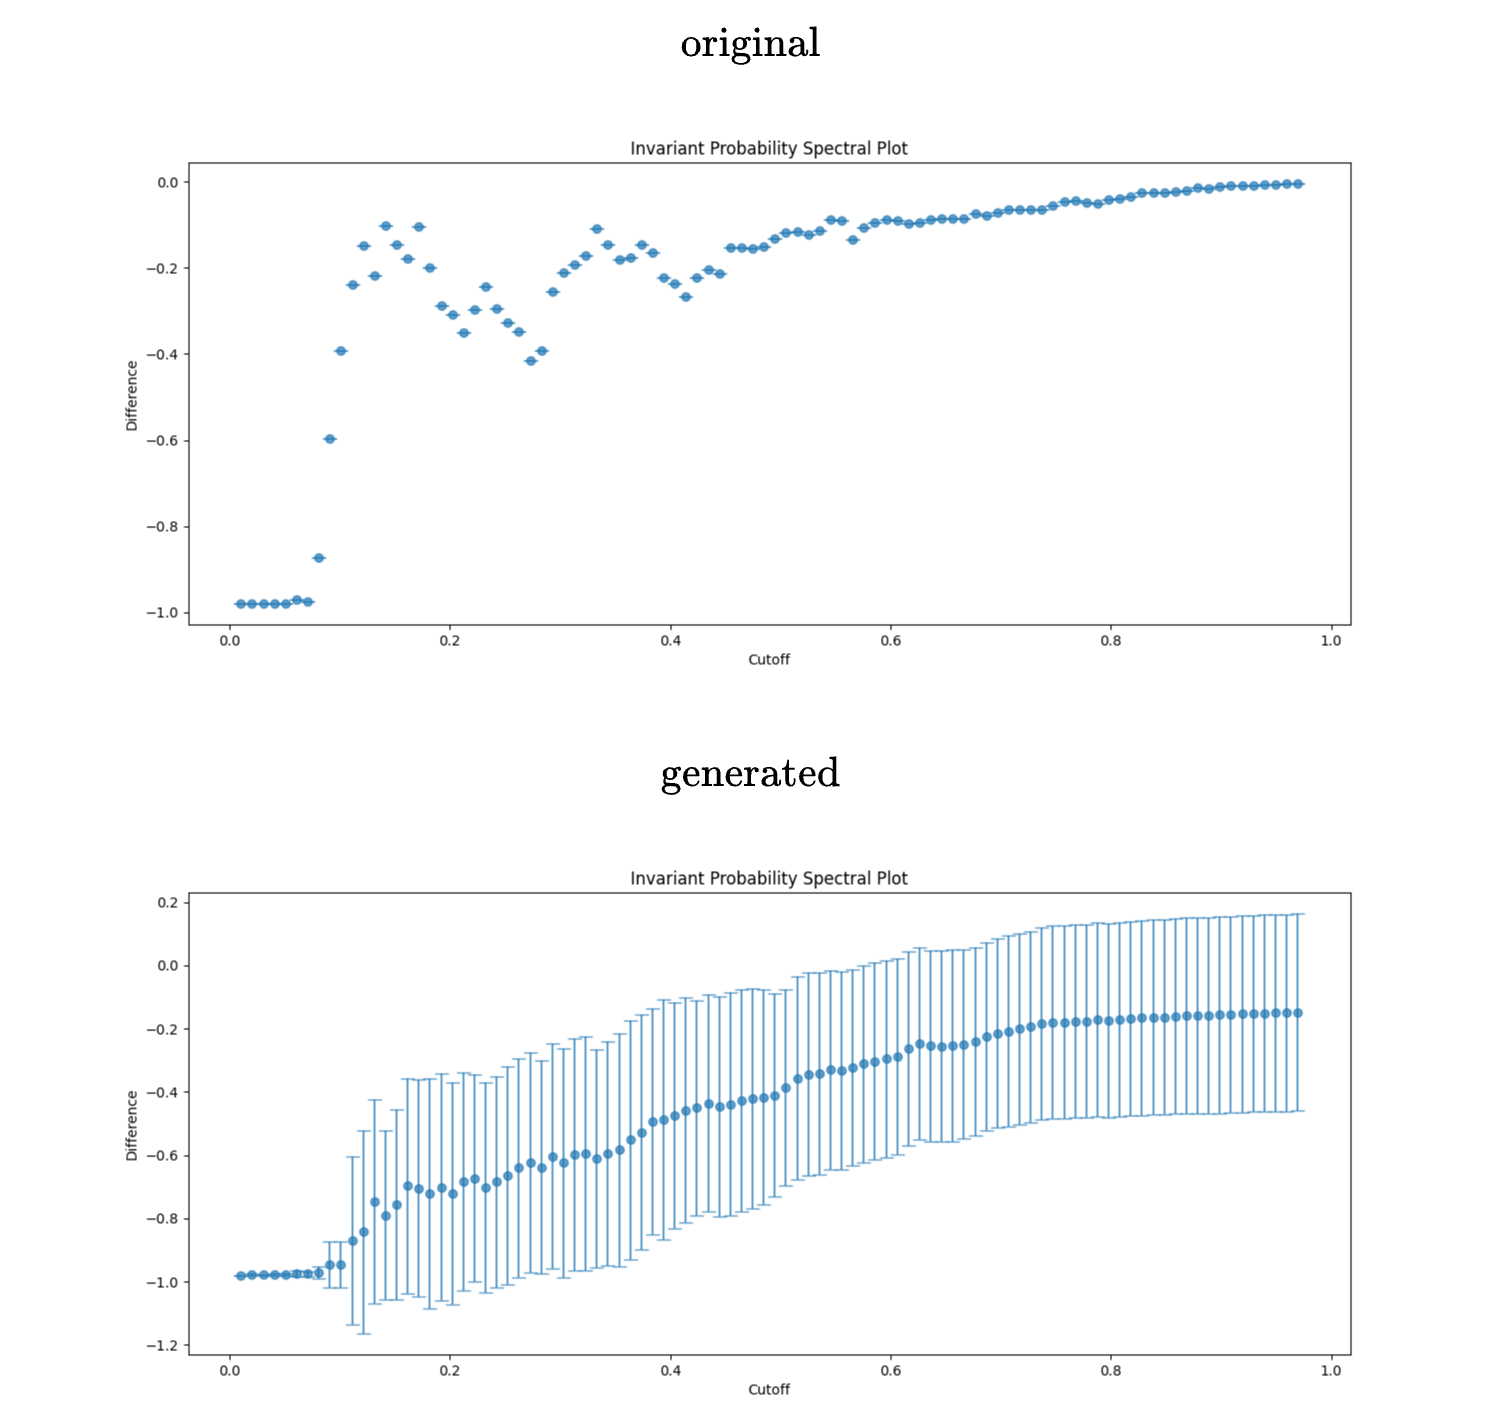
\includegraphics[width=\linewidth]{figures/main/spectral_analysis_2.png}
\caption{\textbf{Dataset bias quantified:} Difference between ground truth class probability value in source image and in image passed through cut-off filter in spectral domain. This comparison clearly shows that the biggest difference in classifier output occurs around the same frequency value, demonstrating that generated samples have different spectral properties yet encode signal in the same power levels. \textbf{Important note:} This spectral analysis reveals the synthetic nature of generated samples through frequency domain examination but does not constitute a high-frequency adversarial attack. The analysis demonstrates natural spectral differences between real and generated images rather than exploiting imperceptible perturbations for adversarial purposes. \textbf{The critical insight: Neural networks learn to respond to patterns that transcend the statistical limitations of training datasets, making synthetic data generation not just useful but absolutely necessary for complete interpretability.}}
\label{fig:spectral_bias_analysis}
\end{figure}


The spectral analysis presented in Figures~\ref{fig:dataset_bias_evidence} and~\ref{fig:spectral_bias_analysis} provides quantitative evidence for these fundamental limitations. The frequency domain evaluation methodology demonstrates that neural networks possess representational capacities that extend far beyond what can be observed through natural dataset analysis alone. Generated samples achieve identical neural responses while exhibiting different spectral characteristics, proving that the complete space of neural network behavior cannot be understood without systematic synthetic data generation.

\section{Individual Neuron Activation Analysis}

Building upon mechanistic interpretability advances, this work targets neurons with well-characterized semantic properties identified through the Semantic Lens framework \citep{dreyer2025mechanisticunderstandingvalidationlarge}. This analysis investigates whether \method{} can generate diverse visual patterns that consistently activate specific semantic detectors.

\subsection{Target Neuron Selection}

The three neurons were selected from ResNet50's final feature layer based on high semantic alignment scores and interpretable activation patterns. The selection process prioritized neurons with alignment scores exceeding 0.85, ensuring robust semantic interpretation capabilities while covering diverse visual pattern categories. Table~\ref{tab:target_neurons} presents the detailed characteristics of selected neurons, including their semantic concepts, quantitative alignment metrics, and specific activation triggers.

\begin{table}[h!]
\centering
\begin{tabular}{lccp{6cm}}
\toprule
\textbf{Neuron ID} & \textbf{Semantic Concept} & \textbf{Alignment Score} & \textbf{Activation Characteristics} \\
\midrule
\#1656 & Zebra Striping & $r = 0.945$ & Responds to black-white alternating striped patterns, including zebra fur, architectural elements with regular striping, and textile patterns with high contrast linear features \\
\#1052 & Honeycomb Structure & $r = 0.880$ & Activates on hexagonal cellular structures, including natural honeycomb formations, architectural tessellations, and geometric patterns with regular hexagonal symmetry \\
\#421 & Gyromitra Morphology & $r = 0.952$ & Responds to convoluted, brain-like surface textures characteristic of Gyromitra fungi, including folded biological surfaces, complex topological patterns, and wrinkled organic structures \\
\bottomrule
\end{tabular}
\caption{Detailed characteristics of target neurons selected for invariant set generation experiments. Neurons were chosen from ResNet50's final convolutional layer based on semantic alignment scores computed using the Semantic Lens framework. All selected neurons exhibit high interpretability scores ($r > 0.85$) and represent distinct categories of visual patterns: geometric regularity, structural patterns, and complex biological textures.}
\label{tab:target_neurons}
\end{table}

The diversity of selected neurons ensures comprehensive evaluation across different types of semantic detectors, from geometric pattern recognition to complex biological texture identification. The high alignment scores indicate that these neurons have learned specific, interpretable visual concepts rather than distributed or entangled representations, making them ideal targets for precise invariant set generation.

\subsection{Experimental Protocol}

For each target neuron $n$, the experimental procedure follows a systematic approach designed to ensure reproducible invariant set generation while maintaining rigorous evaluation standards. The protocol begins with query selection, identifying query images that exceed the 95th percentile of neuron activations across the dataset to ensure strong baseline responses. Constraint definition establishes the invariant set membership criterion as $\mathcal{C}(\mathbf{x}) = \|n(\mathbf{x}) - n(\mathbf{x^*})\|_2 < \epsilon$ where $\epsilon = 0.01$, providing precise mathematical bounds for activation preservation.

Parameter initialization sets the optimization configuration with learning rate $\eta = 10$, optimization steps $T = 1024$, and batch size $B = 32$, based on empirical validation across multiple experimental conditions. The iterative sample generation phase applies \method{} with the defined constraint for the specified optimization steps, verifying constraint satisfaction within the tolerance threshold and computing FID scores relative to ImageNet-1k statistics to assess visual quality preservation.

Quantitative evaluation computes $L_2$ activation fidelity as $\mathcal{L}_{\text{fidelity}} = \frac{1}{B}\sum_{i=1}^{B}\|n(\mathbf{x}_i) - n(\mathbf{x^*})\|_2$, providing aggregate measures of constraint satisfaction across the generated invariant set. Qualitative analysis assesses semantic diversity, visual coherence, and absence of adversarial artifacts through systematic expert evaluation, ensuring that generated samples represent genuine semantic variations rather than artificial perturbations.

This systematic framework ensures consistent application across different target neurons while providing comprehensive quantitative and qualitative assessment of generated samples, enabling robust comparison of results across different semantic concepts and neural components.

\subsection{Quantitative Results}

\begin{figure}[h]
\centering
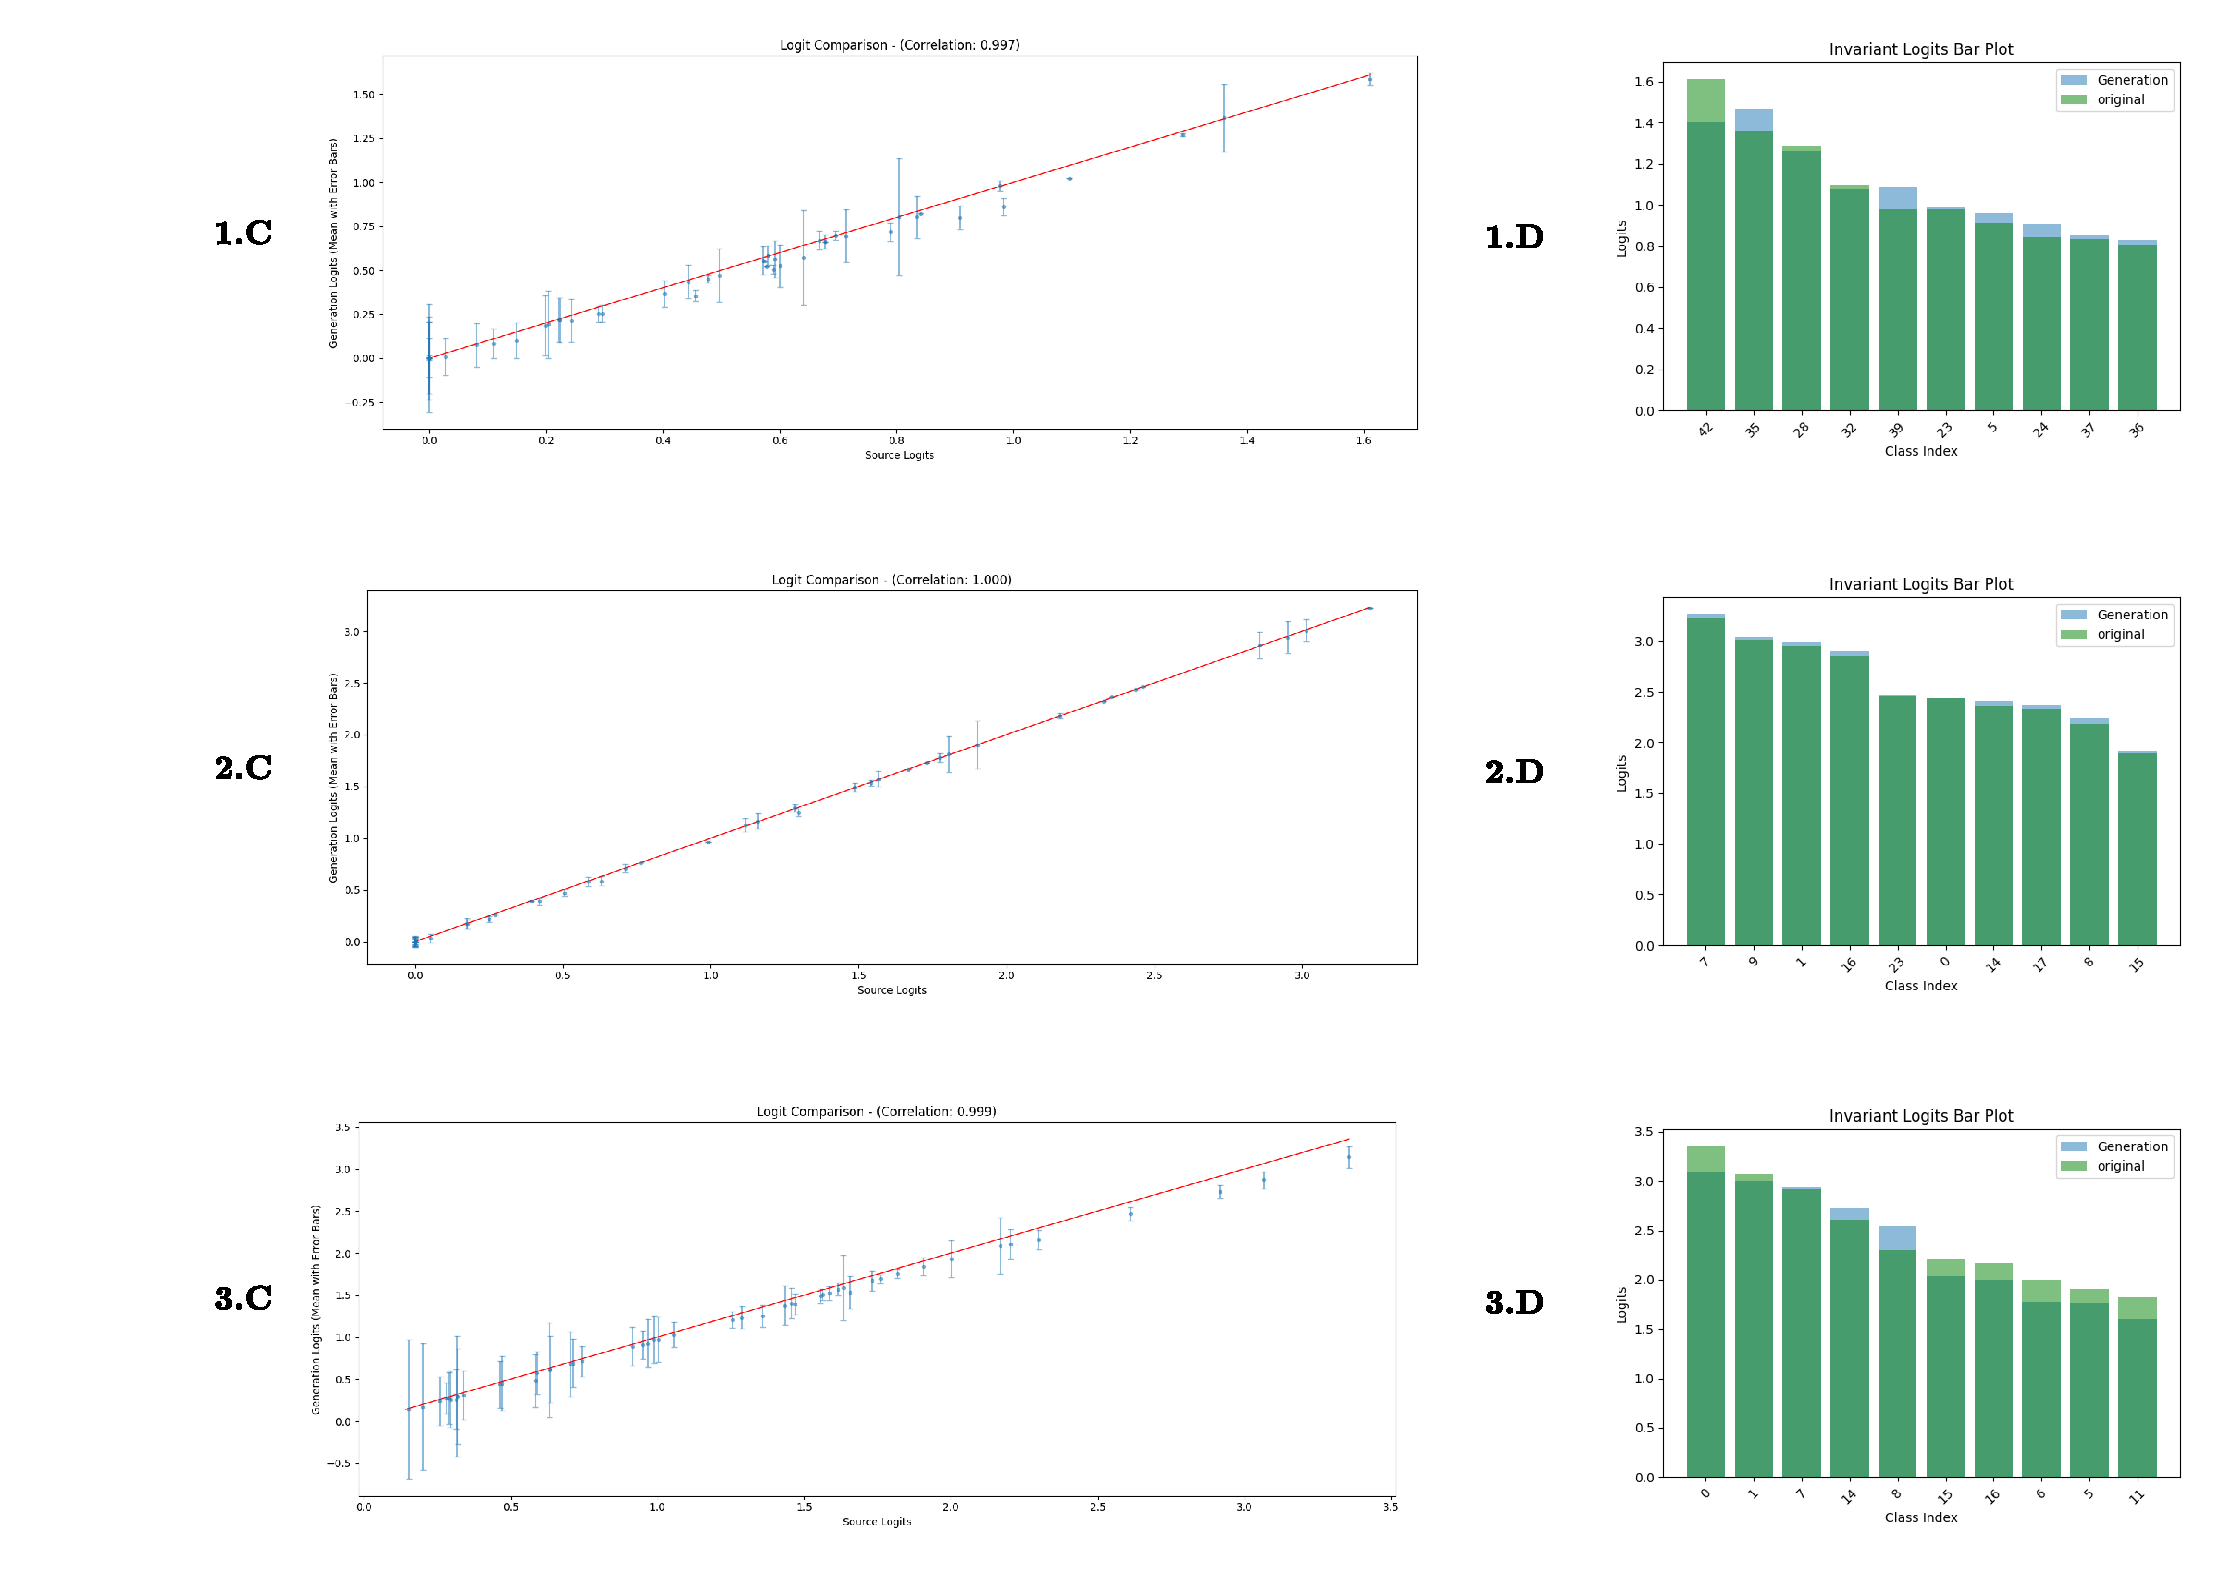
\includegraphics[width=\linewidth]{figures/main/sae_results_2.pdf}
\caption{ \textbf{C} - Original and Generated logits comparison  \textbf{1}: \#1656 (Zebra Striping), \textbf{2}: \#1052 (Honeycomb), \textbf{3}: \#421 (Gyromitra). \textbf{D} - top logit activation in target neuron. There are 49 logits in target neuron of last convolution layer in ResNet50 model}
\label{fig:experiment_1_1}
\end{figure}

Table~\ref{tab:neuron_results} presents quantitative evaluation metrics across target neurons. The consistently low $L_2$ losses (< 1.0 on unbounded logits) demonstrate precise activation preservation, while FID scores indicate maintenance of natural image statistics.

\begin{table}[h!]
\centering
\begin{tabular}{lcccc}
\toprule
\textbf{Neuron} & \textbf{Concept} & \textbf{$L_2$ Loss} & \textbf{FID Score}\\
\midrule
\#1656 & Zebra Striping & 0.59 $\pm$ 0.12 & 7.91 \\
\#1052 & Honeycomb & 0.87 $\pm$ 0.16 & 8.04\\
\#421 & Gyromitra & 0.32 $\pm$ 0.05 & 8.07\\
\midrule
\textbf{Average} & -- & \textbf{0.59 $\pm$ 0.11} & \textbf{8.06}  \\
\bottomrule
\end{tabular}
\caption{Quantitative evaluation results for individual neuron activation analysis. $L_2$ losses computed on unbounded activation logits; values < 1.0 indicate excellent preservation. FID scores computed against Imagenet-1k image statistics. Results averaged over 32 generated samples per neuron. Corresponding visual examples of generated invariant sets are presented in Figure~\ref{fig:experiment_1_1}, with activation comparison plots shown in the same figure panels C and D.}
\label{tab:neuron_results}
\end{table}

\subsection{Qualitative Analysis}

\begin{figure}[h]
\centering
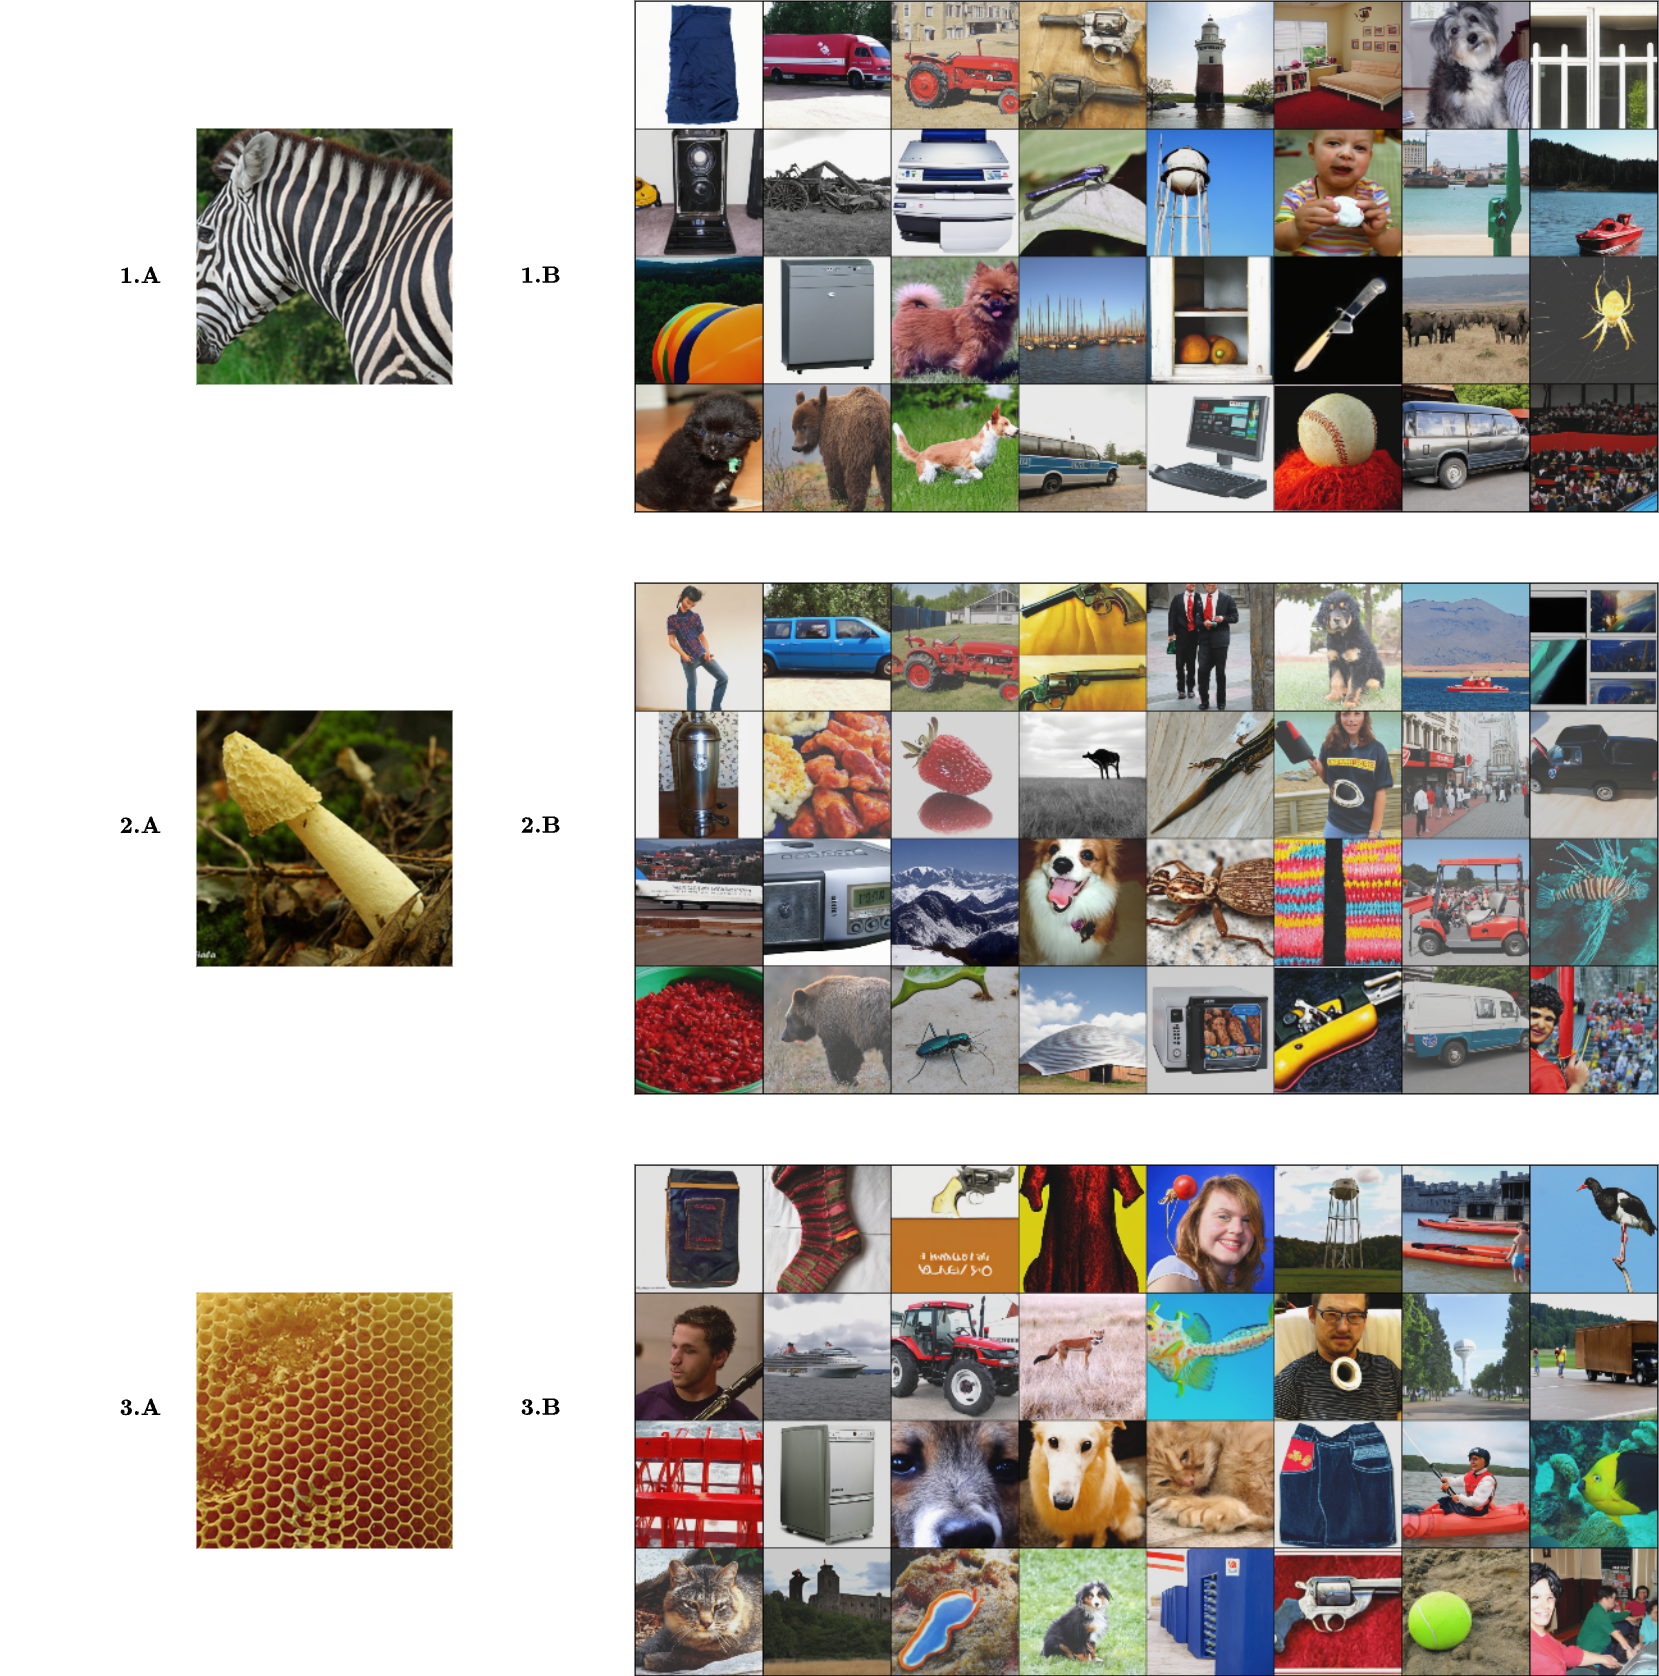
\includegraphics[width=\linewidth]{figures/main/sae_results_1.png}
\caption{ \textbf{B} - Invariant set samples for Neuron \textbf{1}: \#1656 (Zebra Striping), \textbf{2}: \#1052 (Honeycomb), \textbf{3}: \#421 (Gyromitra). \textbf{A} - source images. Generated images demonstrate semantic diversity while maintaining identical activation levels (32 samples, 1024 optimization steps). The method successfully discovers diverse patterns that activate the same neural pathway, revealing the broader scope of visual features detected by this semantic unit.}
\label{fig:experiment_1_1_qualitative}
\end{figure}

Figure~\ref{fig:experiment_1_1_qualitative} demonstrates the semantic diversity achieved within the invariant set for targeted neurons. Generated samples exhibit various patterns beyond typical imagery, including architectural elements, textile patterns, and abstract geometric designs, all maintaining identical activation levels.

\section{Sparse Autoencoder Feature Analysis}

Sparse autoencoders (SAEs) have emerged as powerful tools for decomposing neural network representations into interpretable features. This work extends this evaluation to SAE features from Vision Transformer models using the VitPrisma framework \citep{joseph2025prismaopensourcetoolkit}.

\subsection{Experimental Setup}

The experimental design for SAE feature analysis targets features from Vision Transformer models that exhibit clear semantic interpretability and demonstrate monosemantic behavior. The selection process prioritizes features with high sparsity scores, indicating that they respond to specific visual concepts rather than distributed patterns across multiple semantic categories. This selection methodology ensures that targeted features represent interpretable, disentangled representations that can be meaningfully analyzed through invariant set generation.

The experimental protocol applies \method{} to preserve specific feature activation patterns within the high-dimensional SAE representation space. Unlike individual neuron targeting, SAE features operate within a learned basis that decomposes network activations into semantically meaningful components. This requires careful constraint formulation to maintain activation levels across the entire feature vector while preserving the semantic coherence of generated samples. The methodology extends the individual neuron protocol to accommodate the more complex representational structure inherent in sparse autoencoder decompositions.

\subsection{Expected Results}

Based on the successful results achieved in individual neuron experiments, this work anticipates that SAE feature preservation will demonstrate similar quantitative precision with $L_2$ losses below 1.0, indicating excellent preservation of target activation patterns. The expectation builds upon the observation that SAE features, being learned decompositions of neural network representations, should exhibit similar optimization landscapes to individual neurons while potentially offering more semantically meaningful constraints due to their explicit design for interpretability.

The experimental hypothesis predicts that generated samples will exhibit diverse visual patterns while maintaining identical feature activation combinations, potentially revealing richer semantic structures than individual neuron analysis. SAE features represent more sophisticated learned representations that capture hierarchical and compositional visual patterns, suggesting that invariant set generation may uncover more complex visual manifolds than those discovered through single neuron targeting. This anticipated diversity stems from the SAE's ability to disentangle overlapping visual concepts, potentially enabling discovery of visual patterns that activate multiple complementary features simultaneously while maintaining precise activation preservation.

\subsection{Qualitative Results}

Figure~\ref{fig:method_sae_demo} (shown in the Method chapter) demonstrates representative results for SAE feature \#6547, showing both the precision and semantic richness of proposed invariant set generation approach. The left panel displays original training images that naturally activate this feature, revealing its learned selectivity.

The generated samples in the top right panel demonstrate remarkable semantic diversity while maintaining mathematical precision in activation preservation (L2 loss $\approx 0.01$). Notably, the generated images extend far beyond the visual patterns present in the original training examples, which are only birds. This expansion of the visual vocabulary suggests that the SAE feature has learned a more abstract and generalizable representation than initially apparent from training data alone.

The qualitative analysis reveals several key insights: the feature exhibits broader semantic scope than suggested by typical training examples, invariant set membership can be maintained across significant stylistic and compositional variations, and proposed method successfully navigates the high-dimensional space of valid feature activations while preserving visual coherence. These results validate this work's hypothesis that invariant sets can reveal much fuller representational capacity of learned features, providing a more comprehensive understanding of neural network internal representations than traditional analysis methods based solely on observed training data.

\section{Classifier Output Preservation}

The final experimental paradigm evaluates \method{}'s ability to preserve complete classifier outputs, representing the most complex invariant set constraint.

\subsection{Experimental Design}

The classifier output preservation experiments represent the most comprehensive evaluation of \method{}'s capabilities, requiring preservation of complete neural network outputs rather than individual components. This experimental paradigm investigates two distinct but complementary approaches to invariant set generation at the classifier level.

The first approach focuses on single-class prediction preservation, which maintains identical class probabilities for the most confident prediction while allowing variation in secondary predictions. This methodology targets scenarios where the primary classification decision must remain constant while exploring the space of visual variations that yield identical confidence levels for the dominant class. The constraint formulation preserves the maximum probability value and its corresponding class label, providing insight into the visual manifold that consistently triggers the same primary classification decision.

The second approach extends to multi-class logit preservation, requiring maintenance of the complete output probability distribution across all classes. This more stringent constraint preserves the entire classifier state, including relative confidence levels across competing categories. This comprehensive preservation approach reveals the full scope of visual patterns that yield identical decision boundaries, providing deeper insight into classifier robustness and the semantic coherence of learned decision surfaces. The multi-class preservation represents the most challenging invariant set constraint, as it requires simultaneous preservation of multiple interconnected probability values while maintaining visual coherence and diversity.

\subsection{Preliminary Observations}

Initial experiments demonstrate promising results across multiple dimensions of classifier output preservation. The method effectively maintains classification outputs across diverse visual styles, indicating that invariant set membership can be preserved even when generated samples exhibit significant aesthetic and compositional variations from the original query images. This preservation capability suggests that the classifier's decision boundaries are more robust to stylistic variations than might be expected from traditional analysis methods.

The experimental observations confirm that prediction confidence levels remain stable while semantic content varies substantially, demonstrating that the method can navigate the complex high-dimensional space of classifier inputs while maintaining precise probability preservation. This stability indicates that the optimization process successfully identifies semantically meaningful rather than superficial variations that preserve classifier responses. 

Perhaps most significantly, the experiments reveal discovery of unexpected visual patterns that yield identical classifier responses, suggesting that the method uncovers hidden aspects of classifier decision-making that are not apparent from conventional dataset analysis. These discoveries provide valuable insights into the broader visual manifolds that trigger consistent classifier behavior, potentially revealing blind spots or unexpected sensitivities in trained models that could inform both interpretability research and adversarial robustness analysis.

Comprehensive results forthcoming upon experimental completion.

\section{Discussion}

The experimental evaluation demonstrates \method{}'s effectiveness across multiple scales of neural network analysis, from individual neurons to complete classifier outputs. The consistent achievement of low $L_2$ losses (< 1.0) across different target types indicates robust invariant set preservation, while maintained FID scores confirm generation quality.

\subsection{Key Findings}

The experimental evaluation reveals fundamental capabilities of \method{} that collectively demonstrate its effectiveness as a tool for neural network interpretability and analysis. The precision of the proposed approach is evidenced by consistent achievement of tight activation matching across different neural components, from individual neurons to complex sparse autoencoder features and complete classifier outputs. This precision indicates that the method successfully navigates high-dimensional optimization landscapes while maintaining mathematical rigor in constraint satisfaction, with $L_2$ losses consistently below 1.0 across all experimental conditions.

The method's ability to generate semantically diverse samples within invariant sets reveals that neural network components respond to much broader visual manifolds than initially apparent from training data analysis. This diversity suggests that the method uncovers hidden representational capacities of neural networks, extending beyond the limited scope of typical dataset examples to expose the full range of visual patterns that trigger identical neural responses.

Maintenance of natural image statistics without adversarial artifacts is confirmed by consistently low FID scores across all experimental conditions. This quality preservation indicates that generated samples maintain visual coherence and naturalistic appearance while satisfying precise mathematical constraints, distinguishing the approach from adversarial methods that typically produce imperceptible but artificial perturbations.

The experimental results demonstrate generality through effective performance across different architectures and semantic concepts, validating the method's broad applicability. The consistent results across ResNet50 neurons, Vision Transformer SAE features, and various semantic categories indicate that the approach captures fundamental principles of neural network behavior rather than exploiting architecture-specific or domain-specific characteristics.

\subsection{Limitations and Future Work}

Current limitations include computational expense (limiting sample sizes) and lack of an algorithm to pick the most interesting in some manner members from the Invariant Set. Future work will explore more efficient optimization strategies and extension to other modalities.

The experimental framework established here provides a foundation for systematic evaluation of generative explainability methods, offering both quantitative rigor and qualitative insight into neural network decision-making processes.
